% Options for packages loaded elsewhere
\PassOptionsToPackage{unicode}{hyperref}
\PassOptionsToPackage{hyphens}{url}
%
\documentclass[
  12pt,
  landscape]{article}
\usepackage{lmodern}
\usepackage{amssymb,amsmath}
\usepackage{ifxetex,ifluatex}
\ifnum 0\ifxetex 1\fi\ifluatex 1\fi=0 % if pdftex
  \usepackage[T1]{fontenc}
  \usepackage[utf8]{inputenc}
  \usepackage{textcomp} % provide euro and other symbols
\else % if luatex or xetex
  \usepackage{unicode-math}
  \defaultfontfeatures{Scale=MatchLowercase}
  \defaultfontfeatures[\rmfamily]{Ligatures=TeX,Scale=1}
\fi
% Use upquote if available, for straight quotes in verbatim environments
\IfFileExists{upquote.sty}{\usepackage{upquote}}{}
\IfFileExists{microtype.sty}{% use microtype if available
  \usepackage[]{microtype}
  \UseMicrotypeSet[protrusion]{basicmath} % disable protrusion for tt fonts
}{}
\makeatletter
\@ifundefined{KOMAClassName}{% if non-KOMA class
  \IfFileExists{parskip.sty}{%
    \usepackage{parskip}
  }{% else
    \setlength{\parindent}{0pt}
    \setlength{\parskip}{6pt plus 2pt minus 1pt}}
}{% if KOMA class
  \KOMAoptions{parskip=half}}
\makeatother
\usepackage{xcolor}
\IfFileExists{xurl.sty}{\usepackage{xurl}}{} % add URL line breaks if available
\IfFileExists{bookmark.sty}{\usepackage{bookmark}}{\usepackage{hyperref}}
\hypersetup{
  pdftitle={ECON 21110 - Applied Microeconometrics - Assignment 2},
  pdfauthor={Jack Ogle},
  hidelinks,
  pdfcreator={LaTeX via pandoc}}
\urlstyle{same} % disable monospaced font for URLs
\usepackage[margin=1in]{geometry}
\usepackage{color}
\usepackage{fancyvrb}
\newcommand{\VerbBar}{|}
\newcommand{\VERB}{\Verb[commandchars=\\\{\}]}
\DefineVerbatimEnvironment{Highlighting}{Verbatim}{commandchars=\\\{\}}
% Add ',fontsize=\small' for more characters per line
\usepackage{framed}
\definecolor{shadecolor}{RGB}{248,248,248}
\newenvironment{Shaded}{\begin{snugshade}}{\end{snugshade}}
\newcommand{\AlertTok}[1]{\textcolor[rgb]{0.94,0.16,0.16}{#1}}
\newcommand{\AnnotationTok}[1]{\textcolor[rgb]{0.56,0.35,0.01}{\textbf{\textit{#1}}}}
\newcommand{\AttributeTok}[1]{\textcolor[rgb]{0.77,0.63,0.00}{#1}}
\newcommand{\BaseNTok}[1]{\textcolor[rgb]{0.00,0.00,0.81}{#1}}
\newcommand{\BuiltInTok}[1]{#1}
\newcommand{\CharTok}[1]{\textcolor[rgb]{0.31,0.60,0.02}{#1}}
\newcommand{\CommentTok}[1]{\textcolor[rgb]{0.56,0.35,0.01}{\textit{#1}}}
\newcommand{\CommentVarTok}[1]{\textcolor[rgb]{0.56,0.35,0.01}{\textbf{\textit{#1}}}}
\newcommand{\ConstantTok}[1]{\textcolor[rgb]{0.00,0.00,0.00}{#1}}
\newcommand{\ControlFlowTok}[1]{\textcolor[rgb]{0.13,0.29,0.53}{\textbf{#1}}}
\newcommand{\DataTypeTok}[1]{\textcolor[rgb]{0.13,0.29,0.53}{#1}}
\newcommand{\DecValTok}[1]{\textcolor[rgb]{0.00,0.00,0.81}{#1}}
\newcommand{\DocumentationTok}[1]{\textcolor[rgb]{0.56,0.35,0.01}{\textbf{\textit{#1}}}}
\newcommand{\ErrorTok}[1]{\textcolor[rgb]{0.64,0.00,0.00}{\textbf{#1}}}
\newcommand{\ExtensionTok}[1]{#1}
\newcommand{\FloatTok}[1]{\textcolor[rgb]{0.00,0.00,0.81}{#1}}
\newcommand{\FunctionTok}[1]{\textcolor[rgb]{0.00,0.00,0.00}{#1}}
\newcommand{\ImportTok}[1]{#1}
\newcommand{\InformationTok}[1]{\textcolor[rgb]{0.56,0.35,0.01}{\textbf{\textit{#1}}}}
\newcommand{\KeywordTok}[1]{\textcolor[rgb]{0.13,0.29,0.53}{\textbf{#1}}}
\newcommand{\NormalTok}[1]{#1}
\newcommand{\OperatorTok}[1]{\textcolor[rgb]{0.81,0.36,0.00}{\textbf{#1}}}
\newcommand{\OtherTok}[1]{\textcolor[rgb]{0.56,0.35,0.01}{#1}}
\newcommand{\PreprocessorTok}[1]{\textcolor[rgb]{0.56,0.35,0.01}{\textit{#1}}}
\newcommand{\RegionMarkerTok}[1]{#1}
\newcommand{\SpecialCharTok}[1]{\textcolor[rgb]{0.00,0.00,0.00}{#1}}
\newcommand{\SpecialStringTok}[1]{\textcolor[rgb]{0.31,0.60,0.02}{#1}}
\newcommand{\StringTok}[1]{\textcolor[rgb]{0.31,0.60,0.02}{#1}}
\newcommand{\VariableTok}[1]{\textcolor[rgb]{0.00,0.00,0.00}{#1}}
\newcommand{\VerbatimStringTok}[1]{\textcolor[rgb]{0.31,0.60,0.02}{#1}}
\newcommand{\WarningTok}[1]{\textcolor[rgb]{0.56,0.35,0.01}{\textbf{\textit{#1}}}}
\usepackage{graphicx,grffile}
\makeatletter
\def\maxwidth{\ifdim\Gin@nat@width>\linewidth\linewidth\else\Gin@nat@width\fi}
\def\maxheight{\ifdim\Gin@nat@height>\textheight\textheight\else\Gin@nat@height\fi}
\makeatother
% Scale images if necessary, so that they will not overflow the page
% margins by default, and it is still possible to overwrite the defaults
% using explicit options in \includegraphics[width, height, ...]{}
\setkeys{Gin}{width=\maxwidth,height=\maxheight,keepaspectratio}
% Set default figure placement to htbp
\makeatletter
\def\fps@figure{htbp}
\makeatother
\setlength{\emergencystretch}{3em} % prevent overfull lines
\providecommand{\tightlist}{%
  \setlength{\itemsep}{0pt}\setlength{\parskip}{0pt}}
\setcounter{secnumdepth}{-\maxdimen} % remove section numbering
\usepackage{dcolumn}
\usepackage{float}

\title{ECON 21110 - Applied Microeconometrics - Assignment 2}
\author{Jack Ogle}
\date{}

\begin{document}
\maketitle

Problem 2

\begin{enumerate}
\def\labelenumi{(\alph{enumi})}
\tightlist
\item
  We estimate the population model: \[
  price_i = \beta_0 + \beta_1sqrft_i + \beta_2bdrms_i + \beta_3lotsize_i + U_i
  \]
\end{enumerate}

\begin{table}[!htbp] \centering 
  \caption{Regression Results (a)} 
  \label{} 
\begin{tabular}{@{\extracolsep{5pt}}lc} 
\\[-1.8ex]\hline 
\hline \\[-1.8ex] 
 & \multicolumn{1}{c}{\textit{Dependent variable:}} \\ 
\cline{2-2} 
\\[-1.8ex] & price \\ 
\hline \\[-1.8ex] 
 sqrft & 0.123 \\ 
  & (0.013)$^{***}$ \\ 
  & t = 9.275$^{***}$ \\ 
  & \\ 
 bdrms & 13.853 \\ 
  & (9.010) \\ 
  & t = 1.537 \\ 
  & \\ 
 lotsize & 0.002 \\ 
  & (0.001)$^{***}$ \\ 
  & t = 3.220$^{***}$ \\ 
  & \\ 
 Constant & $-$21.770 \\ 
  & (29.475) \\ 
  & t = $-$0.739 \\ 
  & \\ 
\hline \\[-1.8ex] 
Observations & 88 \\ 
R$^{2}$ & 0.672 \\ 
Adjusted R$^{2}$ & 0.661 \\ 
Residual Std. Error & 59.833 (df = 84) \\ 
F Statistic & 57.460$^{***}$ (df = 3; 84) \\ 
\hline 
\hline \\[-1.8ex] 
\textit{Note:}  & \multicolumn{1}{r}{$^{*}$p$<$0.1; $^{**}$p$<$0.05; $^{***}$p$<$0.01} \\ 
 & \multicolumn{1}{r}{Standard errors in parentheses. T-Statistics below standard errors} \\ 
\end{tabular} 
\end{table}

According to our regression results from Table 1 we can interpret the
following. All other independent variables constant for every increase
in square foot there is an price that is increased by 123 dollars on
average.

All other independent variables constant for every unit increase in lot
size there is an 2 dollar increase in price on average.

All other independent variables constant for every unit increase in
bedrooms there is an 13,853 dollar increase in price on average. This
values is not statistically significant in this regression because the p
value is greater than 0.05.

There is no logical interpretation for the constant as the price of a
house cannot be negative.

\begin{enumerate}
\def\labelenumi{(\alph{enumi})}
\setcounter{enumi}{1}
\item
  The OLS estimate for the parameters in the model we estimated in (a)
  is biased. This is because it violated MLR.4 (the Zero Conditional
  Mean Assumption). There are variables in the error term that are
  correlated with independent variables. For example, variables that
  measure the location of the house is likely correlated with all three
  of the independent variables. If the location is a densely populated
  urban area then it will likely have less square footage, bedrooms, and
  a smaller lot size. Other variables related to the location of the
  house like property tax and average income of the zip-code are also in
  the error term and correlated with the independent variables.
\item
  If we could collect additional data on environmental factors, I would
  include the variables that measure the location of the house. These
  variables include proximity to a large urban area, property tax,
  proximity to a coast, population of the city or town that the house is
  in. I would want to control for all the variables related to location
  of the house because these are correlated with the independent size
  variables and the price. The most important omitted variable that
  would affect the OLS estimator would be property tax the town that the
  house is located in. This would reduced our OVB and make MLR.4 more
  credible. This is because property tax can tell us a lot about the
  location of house. It can tell us if the house is in a wealthy area or
  poor area. If it is in a high crime or low crime area. When we add
  this independent into our regression we can control for crime,
  relative wealth, quality of schools in the area. And when we control
  for these variables we make MLR.4 more credible.
\item
\end{enumerate}

\begin{enumerate}
\def\labelenumi{\roman{enumi})}
\tightlist
\item
  We estimate the population model: \[
  price_i = \beta_0 + \beta_1sqrft_i + \beta_2bdrms_i + \beta_3lotsize_i + \beta_4colonial_i + U_i
  \]

  \begin{table}[!htbp] \centering 
    \caption{Regression Results (d-1)} 
    \label{} 
  \begin{tabular}{@{\extracolsep{5pt}}lc} 
  \\[-1.8ex]\hline 
  \hline \\[-1.8ex] 
   & \multicolumn{1}{c}{\textit{Dependent variable:}} \\ 
  \cline{2-2} 
  \\[-1.8ex] & price \\ 
  \hline \\[-1.8ex] 
   sqrft & 0.124 \\ 
    & (0.013)$^{***}$ \\ 
    & t = 9.314$^{***}$ \\ 
    & \\ 
   bdrms & 11.004 \\ 
    & (9.515) \\ 
    & t = 1.156 \\ 
    & \\ 
   lotsize & 0.002 \\ 
    & (0.001)$^{***}$ \\ 
    & t = 3.230$^{***}$ \\ 
    & \\ 
   colonial & 13.716 \\ 
    & (14.637) \\ 
    & t = 0.937 \\ 
    & \\ 
   Constant & $-$24.127 \\ 
    & (29.603) \\ 
    & t = $-$0.815 \\ 
    & \\ 
  \hline \\[-1.8ex] 
  Observations & 88 \\ 
  R$^{2}$ & 0.676 \\ 
  Adjusted R$^{2}$ & 0.660 \\ 
  Residual Std. Error & 59.877 (df = 83) \\ 
  F Statistic & 43.252$^{***}$ (df = 4; 83) \\ 
  \hline 
  \hline \\[-1.8ex] 
  \textit{Note:}  & \multicolumn{1}{r}{$^{*}$p$<$0.1; $^{**}$p$<$0.05; $^{***}$p$<$0.01} \\ 
   & \multicolumn{1}{r}{Standard errors in parentheses. T-Statistics below standard errors} \\ 
  \end{tabular} 
  \end{table}
\item
  According to our regression results from the table above we can
  interpret the following. All other independent variables constant for
  every increase in square foot there is an price that is increased by
  124 dollars on average.
\end{enumerate}

All other independent variables constant for every unit increase in lot
size there is an 2 dollar increase in price on average.

All other independent variables constant for every unit increase in
bedrooms there is an 11,004 dollar increase in price on average. This
values is not statistically significant in this regression because the p
value is greater than 0.05.

All other independent variables constant if the house is a colonial
style there is an 13,716 dollar increase in price compared to non
colonial style houses on average. This values is not statistically
significant in this regression because the p value is greater than 0.05.

When there are no effects from any independent variables, when they are
all equal to zero the average price is -24,127. However, this value is
not statistically significant in this regression because the p value is
greater than 0.05.

\begin{enumerate}
\def\labelenumi{\roman{enumi})}
\setcounter{enumi}{2}
\tightlist
\item
  \({H_0: \beta_4 = 0}\)
\end{enumerate}

We reject this null hypothesis. However, the coefficient for colonial is
not statistically significant. Adding the colonial binary variable
reduces the effect of bedrooms on price. However, the effect of square
feet and lot size remain constant with the addition. Because the

\begin{enumerate}
\def\labelenumi{(\alph{enumi})}
\setcounter{enumi}{4}
\item
\end{enumerate}

\begin{enumerate}
\def\labelenumi{\roman{enumi})}
\tightlist
\item
  We estimate the population model: \[
  price_i = \beta_0 + \beta_1sqrft_i + \beta_2bdrms_i + \beta_3lotsize_i + \beta_4colonial_i + U_i
  \]
\item
  According to our regression results from Table 1 we can interpret the
  following. All other independent variables constant for every increase
  in square foot there is an price that is increased by 124 dollars on
  average.
\end{enumerate}

All other independent variables constant for every unit increase in lot
size there is an 2 dollar increase in price on average.

All other independent variables constant for every unit increase in
bedrooms there is an 11,004 dollar increase in price on average. This
values is not statistically significant in this regression because the p
value is greater than 0.05.

All other independent variables constant if the house is a colonial
style there is an 13,716 dollar increase in price compared to non
colonial style houses on average. This values is not statistically
significant in this regression because the p value is greater than 0.05.

When there are no effects from any independent variables, when they are
all equal to zero the average price is -24,127. However, this value is
not statistically significant in this regression because the p value is
greater than 0.05.

To find the OVB we need to subtract all coefficients from the original
regression without colonial (\(\hat\beta_1\)) from the coefficients from
the new regression with colonial (\(\tilde\beta_1\)).

OVB for each independent variable: \[
\hat\beta_1- \tilde\beta_1 =  0.123 - 0.124 = -0.001
\] \[
\hat\beta_2- \tilde\beta_2 = 13.853 - 11.004 = 2.849 \\
\] \[
\hat\beta_3- \tilde\beta_3 = 0.002 -0.002 = 0\\
\] I did not understand whether this question was referring to OVB in
the model or just for each coefficient so I assumed that it was for each
coefficient.

\begin{enumerate}
\def\labelenumi{(\alph{enumi})}
\setcounter{enumi}{5}
\item
\end{enumerate}

\begin{enumerate}
\def\labelenumi{\roman{enumi})}
\tightlist
\item
  We estimate the population model: \[
  price_i = \beta_0 + \beta_1sqrft_i + \beta_2bdrms_i + \beta_3lotsize_i +\beta_4colonial_i + \beta_5sqrft_icolonial_i + \beta_6bdrms_icolonial_i + \beta_7lotsize_icolonial_i + U_i
  \]
\end{enumerate}

\begin{table}[H] \centering 
  \caption{Regression Results (f-1)} 
  \label{} 
\begin{tabular}{@{\extracolsep{5pt}}lc} 
\\[-1.8ex]\hline 
\hline \\[-1.8ex] 
 & \multicolumn{1}{c}{\textit{Dependent variable:}} \\ 
\cline{2-2} 
\\[-1.8ex] & price \\ 
\hline \\[-1.8ex] 
 sqrft & 0.090$^{***}$ \\ 
  & (0.024) \\ 
  & \\ 
 bdrms & 11.225 \\ 
  & (20.369) \\ 
  & \\ 
 lotsize & 0.007$^{***}$ \\ 
  & (0.002) \\ 
  & \\ 
 colonial & $-$30.601 \\ 
  & (62.734) \\ 
  & \\ 
 sqrft:colonial & 0.044 \\ 
  & (0.029) \\ 
  & \\ 
 bdrms:colonial & 1.644 \\ 
  & (22.833) \\ 
  & \\ 
 lotsize:colonial & $-$0.006$^{***}$ \\ 
  & (0.002) \\ 
  & \\ 
 Constant & $-$2.874 \\ 
  & (50.810) \\ 
  & \\ 
\hline \\[-1.8ex] 
Observations & 88 \\ 
R$^{2}$ & 0.709 \\ 
Adjusted R$^{2}$ & 0.684 \\ 
Residual Std. Error & 57.758 (df = 80) \\ 
F Statistic & 27.877$^{***}$ (df = 7; 80) \\ 
\hline 
\hline \\[-1.8ex] 
\textit{Note:}  & \multicolumn{1}{r}{$^{*}$p$<$0.1; $^{**}$p$<$0.05; $^{***}$p$<$0.01} \\ 
 & \multicolumn{1}{r}{Standard errors in parentheses} \\ 
\end{tabular} 
\end{table}

\begin{enumerate}
\def\labelenumi{\roman{enumi})}
\setcounter{enumi}{1}
\tightlist
\item
  According to our regression results from the Table above we can
  interpret the following.
\end{enumerate}

All other independent variables constant for every increase in square
foot a colonial house price increases by 134 dollars on average.

All other independent variables constant for every unit increase in lot
size a colonial house price increases 1 dollar in price on average.

All other independent variables constant for every unit increase in
bedrooms a colonial house price increases 12,869 dollar in price on
average. This values is not statistically significant in this regression
because the p value is greater than 0.05.

All other independent variables constant if the house is a colonial
style there is an 30,601 dollar decrease in price compared to non
colonial style houses on average. This values is not statistically
significant in this regression because the p value is greater than 0.05.

When there are no effects from any independent variables, when they are
all equal to zero the average price is -2,874. However, this value is
not statistically significant in this regression because the p value is
greater than 0.05.

\begin{enumerate}
\def\labelenumi{\roman{enumi})}
\setcounter{enumi}{2}
\tightlist
\item
  \({H_0: \beta_5 = 0, H_0: \beta_6 = 0, H_0: \beta_7 = 0 }\)
\end{enumerate}

Our null hypothesis states that there is no evidence that the effect of
house characteristics on price differs by colonial. That in the presence
of colonial we see no difference in the effect of house characteristics.
However, we can see that we can reject the null hypothesis
\(H_0: \beta_6 = 0\) as it equals -0.006 with statistical significance.
This is the only one we can reject because the other results are not
statistically significant. We reject our null hypothesis and should
accept an alternative hypotheses which states that there is a slightly
positive correlation between colonial houses and their lot size. If you
have a colonial house for every unit increase in lot size there is a 1\$
increase in the price of the house on average. This is a result that I
would not expect colonial style houses to differ vary much from other
styles of houses in terms of prices. I would imagine that the prices of
houses colonial or otherwise are affected similarly by house
characteristics.

\begin{enumerate}
\def\labelenumi{(\alph{enumi})}
\setcounter{enumi}{6}
\item
\end{enumerate}

Model (a)

\begin{Shaded}
\begin{Highlighting}[]
\CommentTok{# Graphing the population model }
\KeywordTok{plot}\NormalTok{(modelA, }\DataTypeTok{which=}\DecValTok{1}\NormalTok{)}
\end{Highlighting}
\end{Shaded}

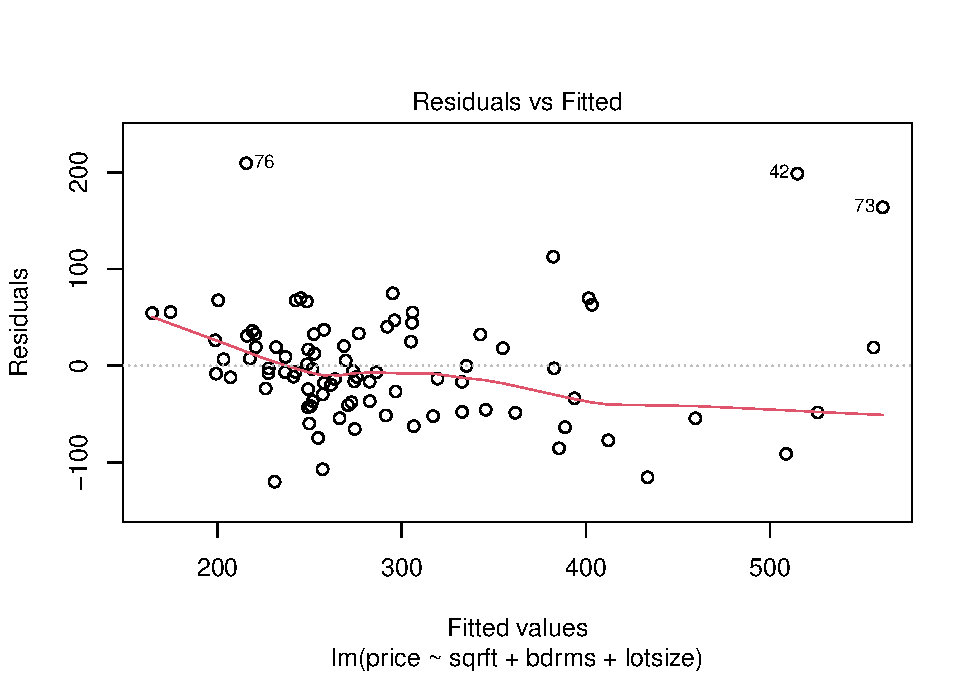
\includegraphics{Ogle_MicroMetricsAssignment_2_Q2_files/figure-latex/unnamed-chunk-5-1.pdf}

Model (d)

\begin{Shaded}
\begin{Highlighting}[]
\CommentTok{# Graphing the population model }
\KeywordTok{plot}\NormalTok{(modelD_}\DecValTok{1}\NormalTok{, }\DataTypeTok{which=}\DecValTok{1}\NormalTok{)}
\end{Highlighting}
\end{Shaded}

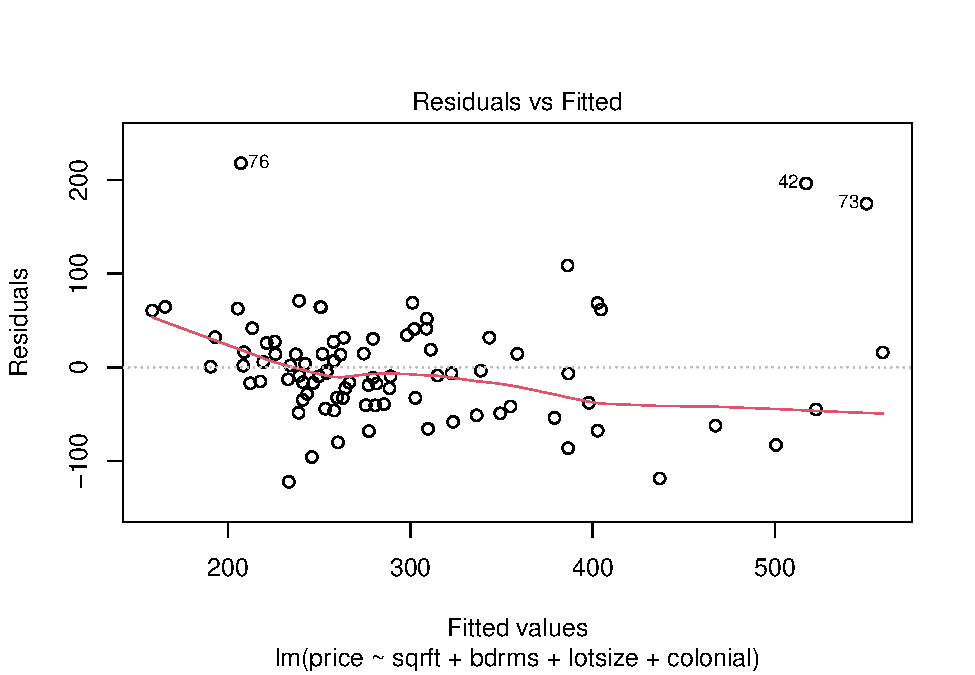
\includegraphics{Ogle_MicroMetricsAssignment_2_Q2_files/figure-latex/unnamed-chunk-6-1.pdf}

Model (f)

\begin{Shaded}
\begin{Highlighting}[]
\CommentTok{# Graphing the population model }
\KeywordTok{plot}\NormalTok{(modelF_}\DecValTok{1}\NormalTok{, }\DataTypeTok{which=}\DecValTok{1}\NormalTok{)}
\end{Highlighting}
\end{Shaded}

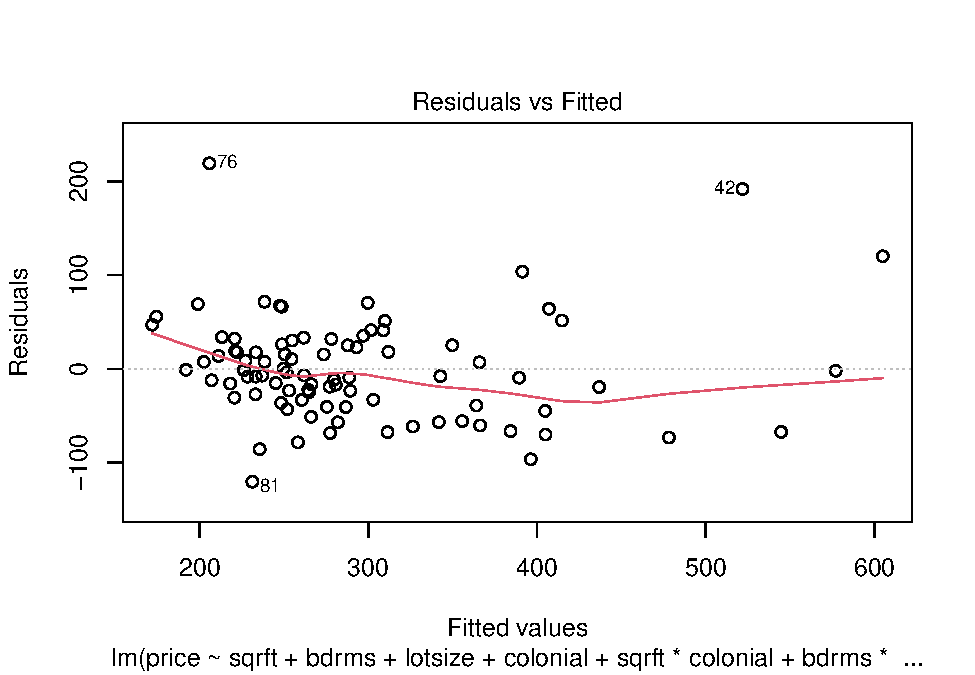
\includegraphics{Ogle_MicroMetricsAssignment_2_Q2_files/figure-latex/unnamed-chunk-7-1.pdf}

If we compare the figures above and the R-squared values for the various
models we learn two important elements about the data and the models
that we created to represent them. All the figures show strong evidence
that our models have heteroskedasticity. As we increase our fitted
values and our independent variables we see a change in the variance of
our residuals. If the models were homoskedastic the residuals would be
evenly distributed even as we increase our independent variables.

By comparing the R-squared values for (a), (d), and (f): 0.672, 0.676,
and 0.709 respectively we know that model (f) has the highest R-squared
and thus fits the data the best.

\begin{enumerate}
\def\labelenumi{(\alph{enumi})}
\setcounter{enumi}{7}
\tightlist
\item
  Heteroskedasticity means that Assumption MLR.5 of homoskedasticity is
  violated. This means that the error variance is not the same across
  all values of the independent variables. Even though under
  heteroskedasticity the estimator \(\hat\beta\) remains unbiased the
  variance of that estimator is biased and we can no longer do
  hypothesis testing. Additionally the standard errors and t-statistics
  we calculated are not correct. Additionally the standard errors are
  higher in the new model and because standard errors are related to
  variance we see a higher variance.
\end{enumerate}

We can see this through a graphic representation of the residuals v. the
fitted values and a BP test

\begin{Shaded}
\begin{Highlighting}[]
\KeywordTok{plot}\NormalTok{(modelA, }\DataTypeTok{which =} \DecValTok{1}\NormalTok{)}
\end{Highlighting}
\end{Shaded}

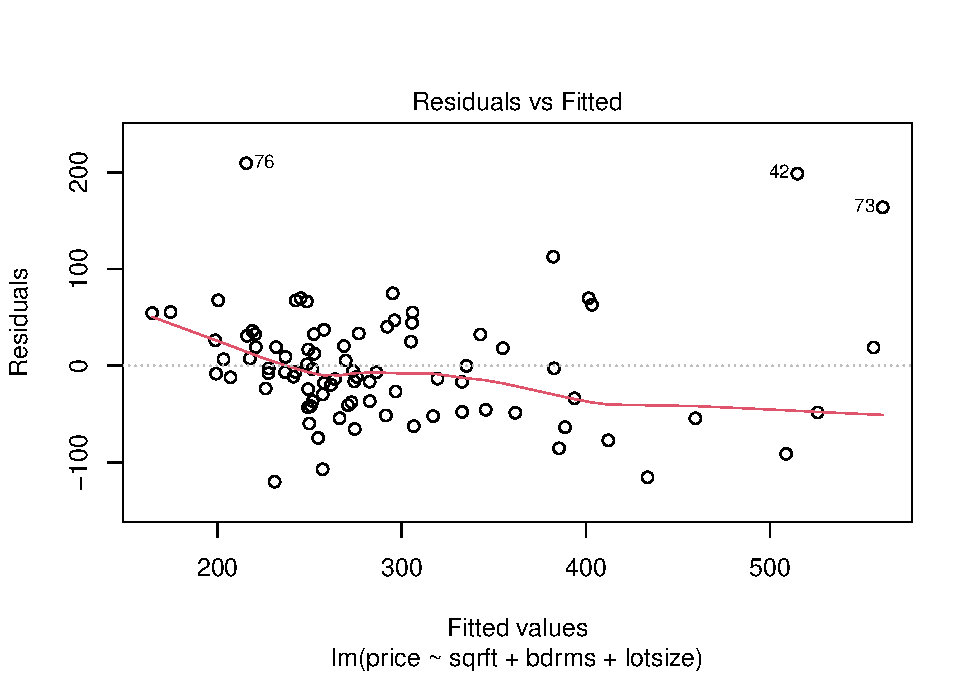
\includegraphics{Ogle_MicroMetricsAssignment_2_Q2_files/figure-latex/unnamed-chunk-8-1.pdf}

The grpahic supports our argument of heteroskedasticity because as we
increase our fitted values and our independent variables we see a change
in the variance of our residuals. If the models were homoskedastic the
residuals would be evenly distributed even as we increase our
independent variables.

Our BP value is 14.092 with three degrees of freedom and a p-value of
0.0028. This is less than our null hypothesis for homoskedasticity which
is BP value equal to 0 with statstical significance. Because we have a
p-value of less than 0.05 we reject the null and there is strong
evidence for heteroskedasticty and a violation of MLR.5.

\begin{enumerate}
\def\labelenumi{(\roman{enumi})}
\item
\end{enumerate}

\begin{table}[H] \centering 
  \caption{Regression Results (I-1)} 
  \label{} 
\begin{tabular}{@{\extracolsep{5pt}}lcc} 
\\[-1.8ex]\hline 
\hline \\[-1.8ex] 
 & \multicolumn{2}{c}{\textit{Dependent variable:}} \\ 
\cline{2-3} 
\\[-1.8ex] & \multicolumn{2}{c}{price} \\ 
 & Non-Robust Std. Errors & Robust Std. Errors \\ 
\\[-1.8ex] & (1) & (2)\\ 
\hline \\[-1.8ex] 
 sqrft & 0.123$^{***}$ & 0.123$^{***}$ \\ 
  & (0.013) & (0.018) \\ 
  & & \\ 
 bdrms & 13.853 & 13.853 \\ 
  & (9.010) & (8.479) \\ 
  & & \\ 
 lotsize & 0.002$^{***}$ & 0.002$^{***}$ \\ 
  & (0.001) & (0.001) \\ 
  & & \\ 
 Constant & $-$21.770 & $-$21.770 \\ 
  & (29.475) & (37.138) \\ 
  & & \\ 
\hline \\[-1.8ex] 
Observations & 88 & 88 \\ 
R$^{2}$ & 0.672 & 0.672 \\ 
Adjusted R$^{2}$ & 0.661 & 0.661 \\ 
Residual Std. Error (df = 84) & 59.833 & 59.833 \\ 
F Statistic (df = 3; 84) & 57.460$^{***}$ & 23.72$^{***}$ \\ 
\hline 
\hline \\[-1.8ex] 
\textit{Note:}  & \multicolumn{2}{r}{$^{*}$p$<$0.1; $^{**}$p$<$0.05; $^{***}$p$<$0.01} \\ 
 & \multicolumn{2}{r}{Standard errors in parentheses} \\ 
\end{tabular} 
\end{table}

For square footage and lot size coefficients the robust standard errors
are larger than the non-robust standard errors. We see a decrease in the
robust standard error for the bedroom coefficient, however, this result
is not statistically significant. We already know that there is
heteroskedasticity present in the model. We use robust standard errors
to correct for the heteroskedascity in the model. Therefore our results
from a remain the same however, because the standard error increases we
have understand that the average distance that the observed values fall
from the regression line increases.

\begin{enumerate}
\def\labelenumi{(\alph{enumi})}
\setcounter{enumi}{9}
\item
\end{enumerate}

\begin{enumerate}
\def\labelenumi{\roman{enumi})}
\tightlist
\item
  We estimate the population model: \[
  lprice_i = \beta_0 + \beta_1sqrft_i + \beta_2bdrms_i + \beta_3lotsize_i + U_i
  \]

  \begin{table}[H] \centering 
    \caption{Regression Results (j-1)} 
    \label{} 
  \begin{tabular}{@{\extracolsep{5pt}}lc} 
  \\[-1.8ex]\hline 
  \hline \\[-1.8ex] 
   & \multicolumn{1}{c}{\textit{Dependent variable:}} \\ 
  \cline{2-2} 
  \\[-1.8ex] & lprice \\ 
  \hline \\[-1.8ex] 
   sqrft & 0.0004$^{***}$ \\ 
    & (0.00004) \\ 
    & \\ 
   bdrms & 0.025 \\ 
    & (0.029) \\ 
    & \\ 
   lotsize & 0.00001$^{***}$ \\ 
    & (0.00000) \\ 
    & \\ 
   Constant & 4.759$^{***}$ \\ 
    & (0.094) \\ 
    & \\ 
  \hline \\[-1.8ex] 
  Observations & 88 \\ 
  R$^{2}$ & 0.622 \\ 
  Adjusted R$^{2}$ & 0.609 \\ 
  Residual Std. Error & 0.190 (df = 84) \\ 
  F Statistic & 46.128$^{***}$ (df = 3; 84) \\ 
  \hline 
  \hline \\[-1.8ex] 
  \textit{Note:}  & \multicolumn{1}{r}{$^{*}$p$<$0.1; $^{**}$p$<$0.05; $^{***}$p$<$0.01} \\ 
   & \multicolumn{1}{r}{Standard errors in parentheses} \\ 
  \end{tabular} 
  \end{table}
\item
  According to our regression results from the table above we can
  interpret the following.
\end{enumerate}

All other independent variables constant for every unit increase in
square footage the house price in dollars increases 0.04\% on average.

All other independent variables constant for every unit increase in
bedrooms the house price in dollars increases 2.5\% on average.

All other independent variables constant for every unit increase in lot
size the house price in dollars increases 0.001\% on average.

When there are no effects from any independent variables, when they are
all equal to zero the average price is 4,759. However, this value is not
statistically significant in this regression because the p value is
greater than 0.05.

\begin{enumerate}
\def\labelenumi{(\alph{enumi})}
\setcounter{enumi}{10}
\tightlist
\item
  Heteroskedasticity means that Assumption MLR.5 of homoskedasticity is
  violated. This means that the error variance is not the same across
  all values of the independent variables. Even though under
  heteroskedasticity the estimator \(\hat\beta\) remains unbiased the
  variance of that estimator is biased and we can no longer do
  hypothesis testing. Additionally the standard errors and t-statistics
  we calculated are not correct. Additionally the standard errors are
  higher in the new model and because standard errors are related to
  variance we see a higher variance.
\end{enumerate}

We can see this through a graphic representation of the residuals v. the
fitted values and a BP test

\begin{Shaded}
\begin{Highlighting}[]
\KeywordTok{plot}\NormalTok{(modelJ_}\DecValTok{1}\NormalTok{, }\DataTypeTok{which =} \DecValTok{1}\NormalTok{)}
\end{Highlighting}
\end{Shaded}

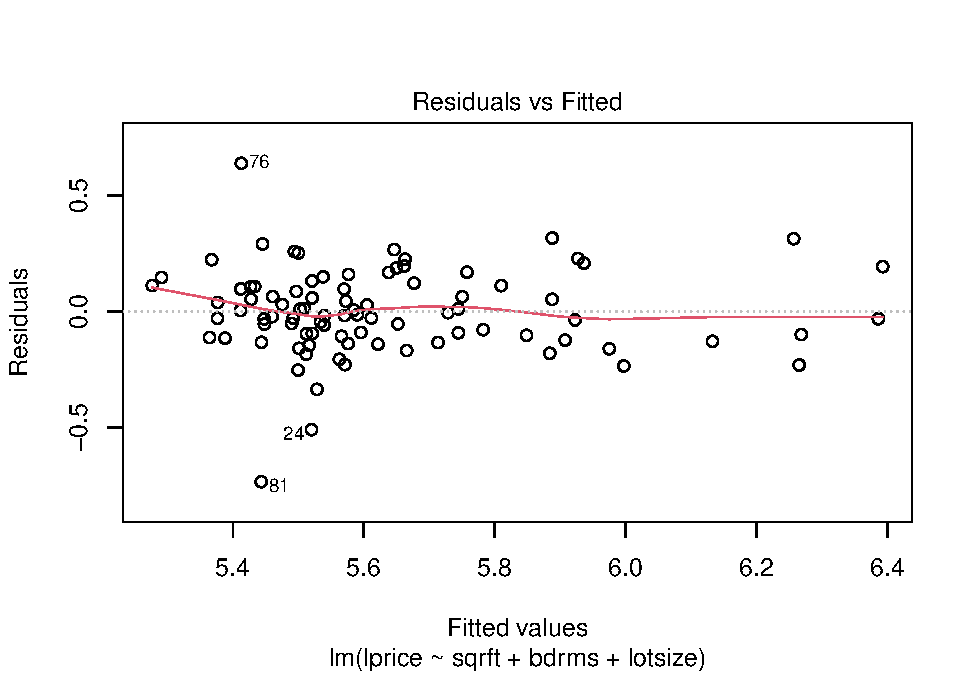
\includegraphics{Ogle_MicroMetricsAssignment_2_Q2_files/figure-latex/unnamed-chunk-12-1.pdf}

The graphic supports our argument of homooskedasticity because as we
increase our fitted values and our independent variables we do not see a
change in the variance of our residuals. The model is homoskedastic
because the residuals are evenly distributed even as we increase our
independent variables.

Our BP value is 3.543 with three degrees of freedom and a p-value of
0.315. Our null hypothesis is that if our BP value is equal to 0 than
there is homoskedasticity in the model. Because we have a p-value of
greater than 0.05 we fail to reject the null and there is strong
evidence for homoskedacitiy and MLR.5 is held. Our boss is right using
log price instead of price fixes our model and makes it homoskedastic.

\begin{enumerate}
\def\labelenumi{(\alph{enumi})}
\setcounter{enumi}{11}
\tightlist
\item
  To see if we should include sqrft in the model we need to calculate
  the OVB for the estimator for bedrooms.
\end{enumerate}

\begin{table}[!htbp] \centering 
  \caption{Regression Results (l-1)} 
  \label{} 
\begin{tabular}{@{\extracolsep{5pt}}lcc} 
\\[-1.8ex]\hline 
\hline \\[-1.8ex] 
 & \multicolumn{2}{c}{\textit{Dependent variable:}} \\ 
\cline{2-3} 
\\[-1.8ex] & \multicolumn{2}{c}{price} \\ 
\\[-1.8ex] & (1) & (2)\\ 
\hline \\[-1.8ex] 
 sqrft & 0.123$^{***}$ &  \\ 
  & (0.013) &  \\ 
  & & \\ 
 bdrms & 13.853 & 57.313$^{***}$ \\ 
  & (9.010) & (10.885) \\ 
  & & \\ 
 lotsize & 0.002$^{***}$ & 0.003$^{***}$ \\ 
  & (0.001) & (0.001) \\ 
  & & \\ 
 Constant & $-$21.770 & 63.262 \\ 
  & (29.475) & (39.620) \\ 
  & & \\ 
\hline \\[-1.8ex] 
Observations & 88 & 88 \\ 
R$^{2}$ & 0.672 & 0.337 \\ 
Adjusted R$^{2}$ & 0.661 & 0.321 \\ 
Residual Std. Error & 59.833 (df = 84) & 84.624 (df = 85) \\ 
F Statistic & 57.460$^{***}$ (df = 3; 84) & 21.585$^{***}$ (df = 2; 85) \\ 
\hline 
\hline \\[-1.8ex] 
\textit{Note:}  & \multicolumn{2}{r}{$^{*}$p$<$0.1; $^{**}$p$<$0.05; $^{***}$p$<$0.01} \\ 
 & \multicolumn{2}{r}{Standard errors in parentheses} \\ 
\end{tabular} 
\end{table}

We can see that the coefficient for bedrooms increase from 12.853 to
57.313. Thus the OVB for this coefficient is -44.46. Omitting sqrft
increases the bedrooms effect on price. And it increases the variance of
that effect on price as we see an increase in the standard error.
Standard error is a statistic that is correlated with variance. And
variance increases. Yes we should included sqrft because we want to
minimize variance and the adjusted r-squared value increases.

\end{document}
